\documentclass[12pt,a4paper]{article}
\usepackage[utf8]{inputenc}
\usepackage[english]{babel}
\usepackage{graphicx}
\usepackage{listings}
\usepackage{xcolor}
\usepackage{hyperref}
\usepackage{geometry}
\usepackage{fancyhdr}
\usepackage{titlesec}
\usepackage{enumitem}

\geometry{margin=2.5cm}
\pagestyle{fancy}
\fancyhf{}
\rhead{Assignment 2 - Energy Management System}
\lhead{Distributed Systems}
\rfoot{Page \thepage}

\definecolor{codegreen}{rgb}{0,0.6,0}
\definecolor{codegray}{rgb}{0.5,0.5,0.5}
\definecolor{codepurple}{rgb}{0.58,0,0.82}
\definecolor{backcolour}{rgb}{0.95,0.95,0.92}

\lstdefinestyle{mystyle}{
    backgroundcolor=\color{backcolour},   
    commentstyle=\color{codegreen},
    keywordstyle=\color{magenta},
    numberstyle=\tiny\color{codegray},
    stringstyle=\color{codepurple},
    basicstyle=\ttfamily\footnotesize,
    breakatwhitespace=false,         
    breaklines=true,                 
    captionpos=b,                    
    keepspaces=true,                 
    numbers=left,                    
    numbersep=5pt,                  
    showspaces=false,                
    showstringspaces=false,
    showtabs=false,                  
    tabsize=2
}

\lstset{style=mystyle}

\title{\textbf{Assignment 2: Energy Management System}\\
\large Message-Oriented Middleware Integration\\
Distributed Systems 2025}
\author{Technical University of Cluj-Napoca}
\date{\today}

\begin{document}

\maketitle
\tableofcontents
\newpage


\section{Introduction}

This document describes the implementation of Assignment 2 for the Distributed Systems course, which extends the Energy Management System from Assignment 1 with Message-Oriented Middleware (MOM) capabilities using RabbitMQ.

\subsection{Project Overview}

The system implements a microservices architecture with asynchronous communication for:
\begin{itemize}
    \item Real-time sensor data processing from IoT devices
    \item Data synchronization between microservices
    \item Energy consumption monitoring and aggregation
    \item Historical data visualization with interactive charts
\end{itemize}

\subsection{Technologies Used}

\begin{itemize}
    \item \textbf{Backend:} Java 17, Spring Boot 3.5.6, Spring AMQP
    \item \textbf{Message Broker:} RabbitMQ 3.13 with Management UI
    \item \textbf{Database:} MySQL 8.0 (separate instances per service)
    \item \textbf{Frontend:} Next.js 15, React 19, TypeScript, Recharts
    \item \textbf{Simulator:} Python 3.9+ with Pika library
    \item \textbf{Infrastructure:} Docker, Docker Compose, Traefik
\end{itemize}

\newpage

\section{System Architecture}

\subsection{Deployment Diagram}

\begin{figure}[h]
\centering
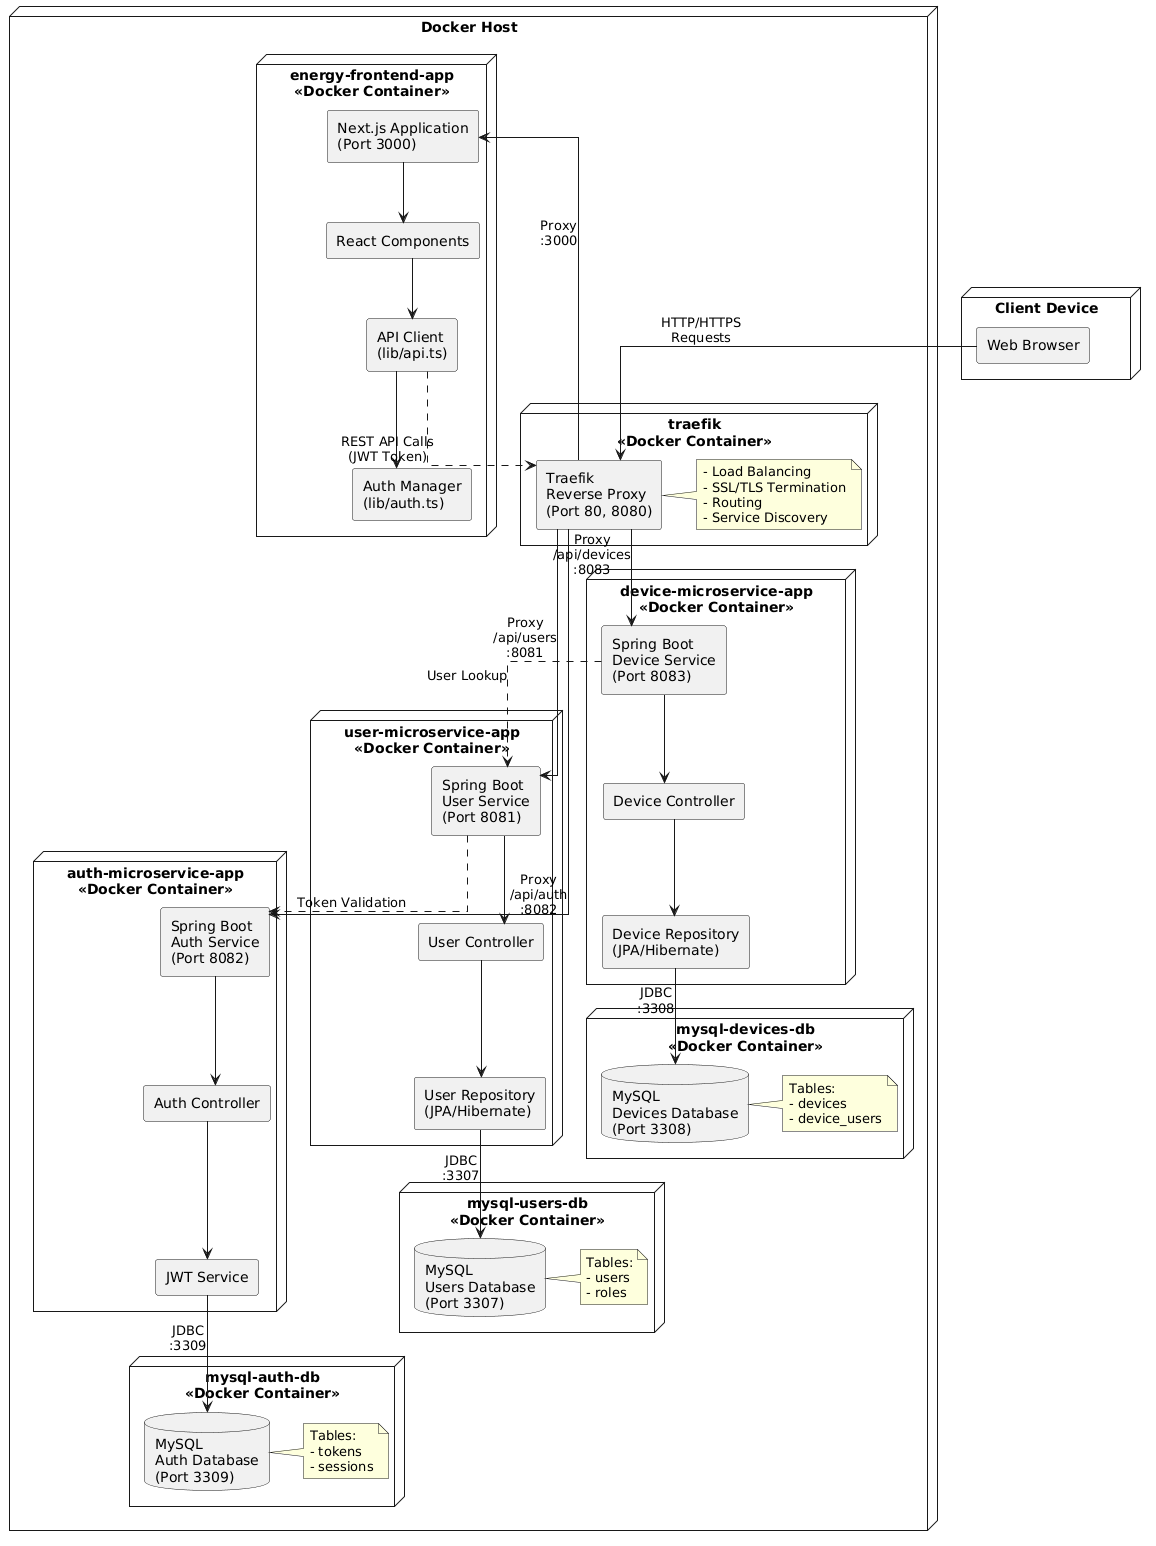
\includegraphics[width=0.9\textwidth]{Deployment diagram.png}
\caption{System Deployment Architecture}
\label{fig:deployment}
\end{figure}

The system consists of the following components:

\begin{enumerate}
    \item \textbf{Traefik Reverse Proxy:} Routes HTTP requests to microservices
    \item \textbf{RabbitMQ Message Broker:} Handles asynchronous communication
    \item \textbf{User Microservice:} Manages user accounts and authentication data
    \item \textbf{Device Microservice:} Manages IoT devices and assignments
    \item \textbf{Monitoring Microservice:} Processes sensor data and aggregates consumption
    \item \textbf{Auth Microservice:} Handles JWT authentication
    \item \textbf{Frontend Application:} Next.js SPA with monitoring dashboard
    \item \textbf{Device Simulator:} Python script simulating IoT sensor data
    \item \textbf{MySQL Databases:} Separate instances for each service
\end{enumerate}

\newpage


\section{Phase 1: Infrastructure Setup}

\subsection{RabbitMQ Configuration}

RabbitMQ was added to the Docker Compose configuration with management UI enabled:

\begin{lstlisting}[language=yaml,caption=docker-compose.yml - RabbitMQ Service]
rabbitmq:
  image: rabbitmq:3.13-management
  container_name: rabbitmq-broker
  restart: unless-stopped
  ports:
    - "5672:5672"   # AMQP protocol port
    - "15672:15672" # Management UI
  environment:
    RABBITMQ_DEFAULT_USER: guest
    RABBITMQ_DEFAULT_PASS: guest
  volumes:
    - rabbitmq-data:/var/lib/rabbitmq
  networks:
    - energy-network
  healthcheck:
    test: ["CMD", "rabbitmq-diagnostics", "ping"]
    interval: 10s
    timeout: 5s
    retries: 5
\end{lstlisting}

\subsection{MySQL Database for Monitoring Service}

A dedicated MySQL instance was created for the Monitoring Microservice:

\begin{lstlisting}[language=yaml,caption=Monitoring Database Configuration]
mysql-monitoring:
  image: mysql:8.0
  container_name: mysql-monitoring-db
  environment:
    MYSQL_ROOT_PASSWORD: root
    MYSQL_DATABASE: energy_monitoring_db
  ports:
    - "3310:3306"
  volumes:
    - mysql-monitoring-data:/var/lib/mysql
  healthcheck:
    test: ["CMD", "mysqladmin", "ping", "-h", "localhost"]
    interval: 10s
    timeout: 5s
    retries: 5
\end{lstlisting}

\subsection{Queue Architecture}

Two main queues were configured in RabbitMQ:

\begin{enumerate}
    \item \textbf{sync\_queue:} For synchronizing user and device data between services
    \item \textbf{sensor\_data\_queue:} For receiving real-time sensor measurements
\end{enumerate}

\newpage


\section{Phase 2: Monitoring Microservice (Java)}

\subsection{Project Structure}

The Monitoring Microservice was implemented in Java using Spring Boot with the following structure:

\begin{verbatim}
monitoring-microservice/
├── src/main/java/com/energy/monitoring/
│   ├── config/
│   │   └── RabbitMQConfig.java
│   ├── controller/
│   │   └── MonitoringController.java
│   ├── dto/
│   │   ├── SensorDataMessage.java
│   │   └── SyncEventMessage.java
│   ├── entity/
│   │   ├── User.java
│   │   ├── Device.java
│   │   └── HourlyConsumption.java
│   ├── listener/
│   │   ├── SensorDataListener.java
│   │   └── SyncQueueListener.java
│   ├── repository/
│   │   ├── UserRepository.java
│   │   ├── DeviceRepository.java
│   │   └── HourlyConsumptionRepository.java
│   └── service/
│       └── ConsumptionAggregationService.java
└── pom.xml
\end{verbatim}

\subsection{Database Schema}

Three main entities were created:

\subsubsection{User Entity}
\begin{lstlisting}[language=Java,caption=User.java]
@Entity
@Table(name = "users")
public class User {
    @Id
    private String id;
    
    @Column(nullable = false, unique = true)
    private String username;
    
    @Column(nullable = false)
    private String email;
    
    @CreationTimestamp
    private LocalDateTime createdAt;
}
\end{lstlisting}


\subsubsection{Device Entity}
\begin{lstlisting}[language=Java,caption=Device.java]
@Entity
@Table(name = "devices")
public class Device {
    @Id
    private String id;
    
    @Column(name = "user_id")
    private String userId;
    
    @Column(nullable = false)
    private String description;
    
    @Column(nullable = false)
    private String address;
    
    @Column(name = "max_hourly_consumption")
    private Double maxHourlyConsumption;
    
    @CreationTimestamp
    private LocalDateTime createdAt;
}
\end{lstlisting}

\subsubsection{HourlyConsumption Entity}
\begin{lstlisting}[language=Java,caption=HourlyConsumption.java]
@Entity
@Table(name = "hourly_consumption")
public class HourlyConsumption {
    @Id
    @GeneratedValue(strategy = GenerationType.IDENTITY)
    private Long id;
    
    @Column(name = "device_id", nullable = false)
    private String deviceId;
    
    @Column(nullable = false)
    private LocalDateTime timestamp;
    
    @Column(name = "consumption_kwh", nullable = false)
    private Double consumptionKwh;
    
    @Column(name = "measurement_count", nullable = false)
    private Integer measurementCount;
    
    @CreationTimestamp
    private LocalDateTime createdAt;
}
\end{lstlisting}


\subsection{RabbitMQ Configuration}

\begin{lstlisting}[language=Java,caption=RabbitMQConfig.java]
@Configuration
public class RabbitMQConfig {
    
    @Bean
    public Queue syncQueue() {
        return new Queue("sync_queue", true);
    }
    
    @Bean
    public Queue sensorDataQueue() {
        return new Queue("sensor_data_queue", true);
    }
    
    @Bean
    public Jackson2JsonMessageConverter messageConverter() {
        ObjectMapper mapper = new ObjectMapper();
        mapper.registerModule(new JavaTimeModule());
        mapper.disable(SerializationFeature.WRITE_DATES_AS_TIMESTAMPS);
        return new Jackson2JsonMessageConverter(mapper);
    }
    
    @Bean
    public RabbitTemplate rabbitTemplate(
            ConnectionFactory connectionFactory,
            Jackson2JsonMessageConverter converter) {
        RabbitTemplate template = new RabbitTemplate(connectionFactory);
        template.setMessageConverter(converter);
        return template;
    }
}
\end{lstlisting}

\subsection{Message Listeners}

\subsubsection{Sync Queue Listener}

Handles synchronization events from User and Device microservices:

\begin{lstlisting}[language=Java,caption=SyncQueueListener.java]
@Component
@Slf4j
public class SyncQueueListener {
    
    @Autowired
    private UserRepository userRepository;
    
    @Autowired
    private DeviceRepository deviceRepository;
    
    @RabbitListener(queues = "sync_queue")
    public void handleSyncEvent(Map<String, Object> message) {
        String event = (String) message.get("event");
        
        if ("USER_CREATED".equals(event) || "USER_UPDATED".equals(event)) {
            handleUserSync(message);
        } else if ("DEVICE_CREATED".equals(event) || "DEVICE_UPDATED".equals(event)) {
            handleDeviceSync(message);
        }
    }
}
\end{lstlisting}


\subsubsection{Sensor Data Listener}

Processes real-time sensor measurements with in-memory buffering:

\begin{lstlisting}[language=Java,caption=SensorDataListener.java - Core Logic]
@Component
@Slf4j
public class SensorDataListener {
    
    // Buffer: deviceId -> hour -> list of measurements
    private final Map<String, Map<String, List<Double>>> buffer = 
        new ConcurrentHashMap<>();
    
    @RabbitListener(queues = "sensor_data_queue")
    public void handleSensorData(SensorDataMessage message) {
        String deviceId = message.getDeviceId();
        Double value = message.getMeasurementValue();
        LocalDateTime timestamp = message.getTimestamp();
        
        // Round to hour
        LocalDateTime hourTimestamp = timestamp
            .truncatedTo(ChronoUnit.HOURS);
        String hourKey = hourTimestamp.toString();
        
        // Add to buffer
        buffer.computeIfAbsent(deviceId, k -> new ConcurrentHashMap<>())
              .computeIfAbsent(hourKey, k -> new ArrayList<>())
              .add(value);
        
        // Check if we have 6 measurements
        List<Double> measurements = buffer.get(deviceId).get(hourKey);
        if (measurements.size() >= 6) {
            aggregateAndSave(deviceId, hourTimestamp, measurements);
            measurements.clear();
        }
    }
    
    private void aggregateAndSave(String deviceId, 
                                  LocalDateTime timestamp, 
                                  List<Double> measurements) {
        double sum = measurements.stream()
            .mapToDouble(Double::doubleValue).sum();
        
        HourlyConsumption consumption = new HourlyConsumption();
        consumption.setDeviceId(deviceId);
        consumption.setTimestamp(timestamp);
        consumption.setConsumptionKwh(sum);
        consumption.setMeasurementCount(measurements.size());
        
        repository.save(consumption);
        log.info("Saved hourly consumption: {} kWh for device {}", 
                 sum, deviceId);
    }
}
\end{lstlisting}


\subsection{REST API Endpoints}

\begin{lstlisting}[language=Java,caption=MonitoringController.java]
@RestController
@RequestMapping("/api/monitoring")
@CrossOrigin(origins = "*")
public class MonitoringController {
    
    @GetMapping("/health")
    public ResponseEntity<String> health() {
        return ResponseEntity.ok("Monitoring service is running");
    }
    
    @GetMapping("/devices")
    public ResponseEntity<List<Device>> getAllDevices() {
        return ResponseEntity.ok(deviceRepository.findAll());
    }
    
    @GetMapping("/devices/{deviceId}/consumption")
    public ResponseEntity<List<HourlyConsumption>> getConsumption(
            @PathVariable String deviceId,
            @RequestParam(required = false) String startDate,
            @RequestParam(required = false) String endDate) {
        
        if (startDate != null && endDate != null) {
            LocalDateTime start = LocalDateTime.parse(startDate);
            LocalDateTime end = LocalDateTime.parse(endDate);
            return ResponseEntity.ok(
                repository.findByDeviceIdAndTimestampBetween(
                    deviceId, start, end));
        }
        
        return ResponseEntity.ok(
            repository.findByDeviceId(deviceId));
    }
}
\end{lstlisting}

\subsection{Docker Configuration}

\begin{lstlisting}[language=yaml,caption=Monitoring Service in docker-compose.yml]
monitoring-microservice:
  build:
    context: ./monitoring-microservice
  container_name: monitoring-microservice-app
  expose:
    - "8084"
  environment:
    DB_HOST: mysql-monitoring
    DB_NAME: energy_monitoring_db
    RABBITMQ_HOST: rabbitmq
  depends_on:
    mysql-monitoring:
      condition: service_healthy
    rabbitmq:
      condition: service_healthy
  labels:
    - "traefik.enable=true"
    - "traefik.http.routers.monitoring.rule=PathPrefix(`/api/monitoring`)"
    - "traefik.http.services.monitoring.loadbalancer.server.port=8084"
\end{lstlisting}

\newpage


\section{Phase 3: Device Simulator (Python)}

\subsection{Implementation}

The device simulator was implemented in Python to generate realistic sensor data:

\begin{lstlisting}[language=Python,caption=simulator.py - Core Logic]
import pika
import json
import time
import random
from datetime import datetime

class DeviceSimulator:
    def __init__(self, config):
        self.device_id = config['device_id']
        self.interval = config.get('interval_seconds', 600)
        self.test_mode = config.get('test_mode', False)
        
        # Connect to RabbitMQ
        credentials = pika.PlainCredentials(
            config['rabbitmq_user'], 
            config['rabbitmq_pass'])
        parameters = pika.ConnectionParameters(
            host=config['rabbitmq_host'],
            port=config['rabbitmq_port'],
            credentials=credentials)
        self.connection = pika.BlockingConnection(parameters)
        self.channel = self.connection.channel()
        self.channel.queue_declare(queue='sensor_data_queue', durable=True)
    
    def generate_measurement(self):
        hour = datetime.now().hour
        
        # Realistic consumption pattern
        if 6 <= hour < 9:  # Morning peak
            base = random.uniform(3.5, 5.0)
        elif 18 <= hour < 22:  # Evening peak
            base = random.uniform(4.0, 5.5)
        elif 22 <= hour or hour < 6:  # Night
            base = random.uniform(1.0, 2.0)
        else:  # Day
            base = random.uniform(2.5, 3.5)
        
        return round(base, 2)
    
    def send_measurement(self):
        value = self.generate_measurement()
        message = {
            'deviceId': self.device_id,
            'measurementValue': value,
            'timestamp': datetime.now().isoformat()
        }
        
        self.channel.basic_publish(
            exchange='',
            routing_key='sensor_data_queue',
            body=json.dumps(message),
            properties=pika.BasicProperties(
                delivery_mode=2,  # Persistent
                content_type='application/json'))
        
        print(f"[{datetime.now()}] Sent: {value} kWh")
    
    def run(self):
        interval = 10 if self.test_mode else self.interval
        print(f"Simulator started (interval: {interval}s)")
        
        while True:
            self.send_measurement()
            time.sleep(interval)
\end{lstlisting}


\subsection{Configuration}

\begin{lstlisting}[language=json,caption=config.json]
{
  "device_id": "e1447307-dbe9-4b1e-a5bf-72248d0cf2bd",
  "rabbitmq_host": "localhost",
  "rabbitmq_port": 5672,
  "rabbitmq_user": "guest",
  "rabbitmq_pass": "guest",
  "interval_seconds": 600,
  "test_mode": true
}
\end{lstlisting}

\textbf{Note:} In test mode, the simulator sends measurements every 10 seconds instead of 600 seconds (10 minutes) for faster testing.

\newpage

\section{Phase 4: User Microservice Modifications}

\subsection{RabbitMQ Integration}

Added RabbitMQ support to publish user creation/update events:

\begin{lstlisting}[language=Java,caption=UserService.java - Event Publishing]
@Service
public class UserService {
    
    @Autowired
    private RabbitTemplate rabbitTemplate;
    
    public UserDTO createUser(CreateUserDTO dto) {
        // Save user to database
        User user = new User();
        user.setId(UUID.randomUUID().toString());
        user.setUsername(dto.getUsername());
        user.setEmail(dto.getEmail());
        // ... set other fields
        
        User savedUser = userRepository.save(user);
        
        // Publish event to RabbitMQ
        Map<String, Object> event = new HashMap<>();
        event.put("event", "USER_CREATED");
        event.put("userId", savedUser.getId());
        event.put("username", savedUser.getUsername());
        event.put("email", savedUser.getEmail());
        
        rabbitTemplate.convertAndSend("sync_queue", event);
        log.info("Published USER_CREATED event for user: {}", 
                 savedUser.getUsername());
        
        return mapToDTO(savedUser);
    }
}
\end{lstlisting}

\subsection{Configuration}

\begin{lstlisting}[caption=application.properties]
spring.rabbitmq.host=rabbitmq
spring.rabbitmq.port=5672
spring.rabbitmq.username=guest
spring.rabbitmq.password=guest
\end{lstlisting}

\newpage


\section{Phase 5: Device Microservice Modifications}

\subsection{RabbitMQ Integration}

Similar to User Microservice, Device Microservice publishes events:

\begin{lstlisting}[language=Java,caption=DeviceService.java - Event Publishing]
@Service
public class DeviceService {
    
    @Autowired
    private RabbitTemplate rabbitTemplate;
    
    public DeviceDTO createDevice(CreateDeviceDTO dto) {
        Device device = new Device();
        device.setId(UUID.randomUUID().toString());
        device.setDescription(dto.getDescription());
        device.setAddress(dto.getAddress());
        device.setMaximumHourlyConsumption(dto.getMaximumHourlyConsumption());
        device.setUserId(dto.getUserId());
        
        Device savedDevice = deviceRepository.save(device);
        
        // Publish event to RabbitMQ
        Map<String, Object> event = new HashMap<>();
        event.put("event", "DEVICE_CREATED");
        event.put("deviceId", savedDevice.getId());
        event.put("userId", savedDevice.getUserId());
        event.put("description", savedDevice.getDescription());
        event.put("address", savedDevice.getAddress());
        event.put("maxHourlyConsumption", 
                  savedDevice.getMaximumHourlyConsumption());
        
        rabbitTemplate.convertAndSend("sync_queue", event);
        log.info("Published DEVICE_CREATED event for device: {}", 
                 savedDevice.getId());
        
        return mapToDTO(savedDevice);
    }
}
\end{lstlisting}

\newpage

\section{Phase 6: Frontend Monitoring Dashboard}

\subsection{Implementation}

A new monitoring page was created with interactive charts:

\begin{lstlisting}[language=JavaScript,caption=monitoring/page.tsx - Key Features]
export default function MonitoringPage() {
  const [devices, setDevices] = useState([]);
  const [selectedDevice, setSelectedDevice] = useState("");
  const [selectedDate, setSelectedDate] = useState(new Date());
  const [consumptionData, setConsumptionData] = useState([]);
  const [chartType, setChartType] = useState("line");
  
  const fetchConsumptionData = async () => {
    const startDate = new Date(selectedDate);
    startDate.setHours(0, 0, 0, 0);
    
    const endDate = new Date(selectedDate);
    endDate.setHours(23, 59, 59, 999);
    
    const response = await fetch(
      `${API_BASE_URL}/api/monitoring/devices/${selectedDevice}/consumption?startDate=${startDate.toISOString()}&endDate=${endDate.toISOString()}`
    );
    
    const data = await response.json();
    setConsumptionData(data);
  };
  
  return (
    <div>
      {/* Device Selector */}
      <Select value={selectedDevice} onValueChange={setSelectedDevice}>
        {devices.map(device => (
          <SelectItem key={device.id} value={device.id}>
            {device.description}
          </SelectItem>
        ))}
      </Select>
      
      {/* Date Picker */}
      <Calendar 
        selected={selectedDate} 
        onSelect={setSelectedDate} 
      />
      
      {/* Chart */}
      <ResponsiveContainer width="100%" height={400}>
        <LineChart data={chartData}>
          <XAxis dataKey="time" />
          <YAxis />
          <Tooltip />
          <Line dataKey="consumption" stroke="#8884d8" />
        </LineChart>
      </ResponsiveContainer>
    </div>
  );
}
\end{lstlisting}


\subsection{Features}

\begin{itemize}
    \item \textbf{Device Selection:} Dropdown to select from available devices
    \item \textbf{Date Picker:} Calendar widget to select date for viewing data
    \item \textbf{Chart Types:} Toggle between Line Chart and Bar Chart
    \item \textbf{Statistics:} Display total, average, and peak consumption
    \item \textbf{Real-time Updates:} Load button to fetch latest data
\end{itemize}

\newpage

\section{Message Flow Architecture}

\subsection{User/Device Synchronization Flow}

\begin{verbatim}
1. User creates device in Frontend
   ↓
2. Frontend → POST /api/devices (via Traefik)
   ↓
3. Device Microservice:
   - Saves device to MySQL
   - Publishes DEVICE_CREATED event to sync_queue
   ↓
4. RabbitMQ routes message to sync_queue
   ↓
5. Monitoring Microservice:
   - SyncQueueListener receives event
   - Saves device copy to local MySQL
   - Logs: "Synced device: [device-id]"
\end{verbatim}

\subsection{Sensor Data Processing Flow}

\begin{verbatim}
1. Device Simulator generates measurement
   ↓
2. Simulator → RabbitMQ (sensor_data_queue)
   Message: {
     "deviceId": "abc-123",
     "measurementValue": 3.45,
     "timestamp": "2025-11-19T10:30:00"
   }
   ↓
3. RabbitMQ routes to sensor_data_queue
   ↓
4. Monitoring Microservice:
   - SensorDataListener receives message
   - Adds to in-memory buffer
   - Buffer structure: Map<deviceId, Map<hour, List<values>>>
   ↓
5. When buffer reaches 6 measurements:
   - Calculate sum: Σ(measurements)
   - Create HourlyConsumption entity
   - Save to MySQL
   - Clear buffer for that hour
   - Log: "Saved hourly consumption: X kWh"
   ↓
6. Frontend requests data:
   GET /api/monitoring/devices/{id}/consumption?startDate=...&endDate=...
   ↓
7. Monitoring Controller:
   - Query HourlyConsumption table
   - Filter by deviceId and timestamp range
   - Return JSON array
   ↓
8. Frontend:
   - Receives consumption data
   - Transforms to chart format
   - Renders Line/Bar chart with Recharts
\end{verbatim}

\newpage


\section{Testing and Validation}

\subsection{Test Scenario 1: Device Creation and Synchronization}

\textbf{Objective:} Verify that device creation triggers synchronization to Monitoring service.

\textbf{Steps:}
\begin{enumerate}
    \item Login as admin at \texttt{http://localhost:3000/dashboard/login}
    \item Navigate to Devices page
    \item Click "Create Device" button
    \item Fill in form:
    \begin{itemize}
        \item Description: "Smart Meter Test 001"
        \item Address: "192.168.1.100"
        \item Max Hourly Consumption: 15.0 kWh
        \item Assign to user: admin
    \end{itemize}
    \item Click "Save"
\end{enumerate}

\textbf{Expected Results:}
\begin{itemize}
    \item Device appears in devices list
    \item RabbitMQ Management UI shows message in \texttt{sync\_queue}
    \item Monitoring service logs: "Synced device: Smart Meter Test 001"
    \item Device visible in Monitoring database
\end{itemize}

\textbf{Verification Commands:}
\begin{lstlisting}[language=bash]
# Check RabbitMQ queue
curl -u guest:guest http://localhost:15672/api/queues/%2F/sync_queue

# Check Monitoring database
docker exec -it mysql-monitoring-db mysql -u root -proot \
  energy_monitoring_db -e "SELECT * FROM devices;"

# Check Monitoring service logs
docker logs monitoring-microservice-app | grep "Synced device"
\end{lstlisting}

\subsection{Test Scenario 2: Sensor Data Aggregation}

\textbf{Objective:} Verify that simulator sends data and Monitoring service aggregates it correctly.

\textbf{Steps:}
\begin{enumerate}
    \item Configure simulator with device ID from Test 1
    \item Edit \texttt{device-simulator/config.json}:
\begin{lstlisting}[language=json]
{
  "device_id": "e1447307-dbe9-4b1e-a5bf-72248d0cf2bd",
  "test_mode": true
}
\end{lstlisting}
    \item Start simulator: \texttt{python device-simulator/simulator.py}
    \item Wait 60 seconds (6 measurements × 10s)
\end{enumerate}

\textbf{Expected Results:}
\begin{itemize}
    \item Simulator logs show 6 measurements sent
    \item RabbitMQ shows messages processed from \texttt{sensor\_data\_queue}
    \item Monitoring service logs: "Saved hourly consumption: X kWh"
    \item Database contains new \texttt{hourly\_consumption} record
\end{itemize}


\textbf{Verification Commands:}
\begin{lstlisting}[language=bash]
# Check simulator output
# Should show: [2025-11-19 10:30:00] Sent: 3.45 kWh

# Check RabbitMQ messages
curl -u guest:guest \
  http://localhost:15672/api/queues/%2F/sensor_data_queue

# Check aggregated data in database
docker exec -it mysql-monitoring-db mysql -u root -proot \
  energy_monitoring_db -e \
  "SELECT * FROM hourly_consumption ORDER BY timestamp DESC LIMIT 5;"

# Expected output:
# +----+----------+---------------------+-----------------+-------+
# | id | device_id| timestamp           | consumption_kwh | count |
# +----+----------+---------------------+-----------------+-------+
# |  1 | abc-123  | 2025-11-19 10:00:00 |           20.38 |     6 |
# +----+----------+---------------------+-----------------+-------+

# Check Monitoring service logs
docker logs monitoring-microservice-app --tail 20
\end{lstlisting}

\subsection{Test Scenario 3: Frontend Chart Visualization}

\textbf{Objective:} Verify that frontend displays consumption data correctly.

\textbf{Steps:}
\begin{enumerate}
    \item Navigate to \texttt{http://localhost:3000/dashboard}
    \item Click "Energy Monitoring" button in Quick Actions
    \item Select device: "Smart Meter Test 001"
    \item Select date: Today's date (19 November 2025)
    \item Click "Load Data" button
\end{enumerate}

\textbf{Expected Results:}
\begin{itemize}
    \item Chart displays with consumption data
    \item Statistics cards show:
    \begin{itemize}
        \item Total Consumption: Sum of all hourly values
        \item Average Consumption: Mean of hourly values
        \item Peak Consumption: Maximum hourly value
    \end{itemize}
    \item X-axis shows hours (0-23)
    \item Y-axis shows consumption in kWh
    \item Tooltip displays exact values on hover
\end{itemize}

\textbf{API Verification:}
\begin{lstlisting}[language=bash]
# Test API endpoint directly
curl "http://localhost/api/monitoring/devices/e1447307-dbe9-4b1e-a5bf-72248d0cf2bd/consumption?startDate=2025-11-19T00:00:00.000Z&endDate=2025-11-19T23:59:59.999Z"

# Expected response:
# [
#   {
#     "timestamp": "2025-11-19T10:00:00",
#     "consumption": 20.38,
#     "measurementCount": 6
#   }
# ]
\end{lstlisting}

\newpage


\subsection{Test Scenario 4: Complete End-to-End Flow}

\textbf{Objective:} Demonstrate complete system functionality from device creation to chart visualization.

\textbf{Complete Test Script:}

\begin{lstlisting}[language=bash,caption=complete\_test.sh]
#!/bin/bash

echo "=== COMPLETE E2E TEST ==="
echo ""

# Step 1: Create test user
echo "Step 1: Creating test user..."
curl -X POST http://localhost/api/users \
  -H "Content-Type: application/json" \
  -H "Authorization: Bearer $ADMIN_TOKEN" \
  -d '{
    "username": "testuser",
    "password": "test123",
    "email": "test@energy.ro",
    "fullName": "Test User",
    "role": "CLIENT"
  }'

USER_ID=$(curl -s http://localhost/api/users | \
  jq -r '.[] | select(.username=="testuser") | .id')
echo "Created user with ID: $USER_ID"
echo ""

# Step 2: Create test device
echo "Step 2: Creating test device..."
DEVICE_RESPONSE=$(curl -X POST http://localhost/api/devices \
  -H "Content-Type: application/json" \
  -H "Authorization: Bearer $ADMIN_TOKEN" \
  -d "{
    \"description\": \"E2E Test Device\",
    \"address\": \"192.168.1.200\",
    \"maximumHourlyConsumption\": 20.0,
    \"userId\": \"$USER_ID\"
  }")

DEVICE_ID=$(echo $DEVICE_RESPONSE | jq -r '.id')
echo "Created device with ID: $DEVICE_ID"
echo ""

# Step 3: Verify sync in Monitoring DB
echo "Step 3: Verifying device sync..."
sleep 2
docker exec mysql-monitoring-db mysql -u root -proot \
  energy_monitoring_db -e \
  "SELECT * FROM devices WHERE id='$DEVICE_ID';"
echo ""

# Step 4: Configure and start simulator
echo "Step 4: Configuring simulator..."
cat > device-simulator/config.json <<EOF
{
  "device_id": "$DEVICE_ID",
  "rabbitmq_host": "localhost",
  "rabbitmq_port": 5672,
  "rabbitmq_user": "guest",
  "rabbitmq_pass": "guest",
  "test_mode": true
}
EOF

echo "Starting simulator for 60 seconds..."
timeout 60 python device-simulator/simulator.py &
SIMULATOR_PID=$!
sleep 65
echo ""

# Step 5: Verify aggregated data
echo "Step 5: Checking aggregated consumption data..."
docker exec mysql-monitoring-db mysql -u root -proot \
  energy_monitoring_db -e \
  "SELECT * FROM hourly_consumption WHERE device_id='$DEVICE_ID';"
echo ""

# Step 6: Test API endpoint
echo "Step 6: Testing API endpoint..."
TODAY=$(date -u +"%Y-%m-%dT00:00:00.000Z")
TOMORROW=$(date -u -d "tomorrow" +"%Y-%m-%dT00:00:00.000Z")

curl "http://localhost/api/monitoring/devices/$DEVICE_ID/consumption?startDate=$TODAY&endDate=$TOMORROW" | jq
echo ""

echo "=== TEST COMPLETE ==="
echo "Now open http://localhost:3000/dashboard/monitoring"
echo "Select device: E2E Test Device"
echo "Select date: Today"
echo "Click: Load Data"
\end{lstlisting}


\textbf{Expected Output:}

\begin{verbatim}
=== COMPLETE E2E TEST ===

Step 1: Creating test user...
Created user with ID: 550e8400-e29b-41d4-a716-446655440000

Step 2: Creating test device...
Created device with ID: e1447307-dbe9-4b1e-a5bf-72248d0cf2bd

Step 3: Verifying device sync...
+--------------------------------------+----------+------------------+
| id                                   | user_id  | description      |
+--------------------------------------+----------+------------------+
| e1447307-dbe9-4b1e-a5bf-72248d0cf2bd | 550e...  | E2E Test Device  |
+--------------------------------------+----------+------------------+

Step 4: Configuring simulator...
Starting simulator for 60 seconds...
[2025-11-19 10:30:00] Sent: 3.45 kWh
[2025-11-19 10:30:10] Sent: 3.78 kWh
[2025-11-19 10:30:20] Sent: 3.21 kWh
[2025-11-19 10:30:30] Sent: 3.92 kWh
[2025-11-19 10:30:40] Sent: 3.56 kWh
[2025-11-19 10:30:50] Sent: 3.46 kWh

Step 5: Checking aggregated consumption data...
+----+----------+---------------------+-----------------+-------+
| id | device_id| timestamp           | consumption_kwh | count |
+----+----------+---------------------+-----------------+-------+
|  1 | e1447... | 2025-11-19 10:00:00 |           21.38 |     6 |
+----+----------+---------------------+-----------------+-------+

Step 6: Testing API endpoint...
[
  {
    "timestamp": "2025-11-19T10:00:00",
    "consumption": 21.38,
    "measurementCount": 6
  }
]

=== TEST COMPLETE ===
\end{verbatim}

\newpage

\section{Theoretical Questions}

\subsection{What is Message-Oriented Middleware (MOM)?}

Message-Oriented Middleware (MOM) is a software infrastructure that enables asynchronous communication between distributed applications by exchanging messages through a message broker.

\textbf{Key Characteristics:}
\begin{itemize}
    \item \textbf{Asynchronous Communication:} Sender and receiver don't need to interact simultaneously
    \item \textbf{Loose Coupling:} Services don't need to know about each other's implementation
    \item \textbf{Reliability:} Messages can be persisted and guaranteed delivery
    \item \textbf{Scalability:} Easy to add new consumers or producers
\end{itemize}

\textbf{Examples:}
\begin{itemize}
    \item RabbitMQ (AMQP protocol)
    \item Apache Kafka (distributed streaming)
    \item ActiveMQ (JMS implementation)
    \item Amazon SQS (cloud-based)
    \item Redis Pub/Sub
\end{itemize}

\textbf{Advantages:}
\begin{itemize}
    \item Decoupling of services
    \item Load balancing and scalability
    \item Fault tolerance and reliability
    \item Buffering during traffic spikes
    \item Support for multiple communication patterns
\end{itemize}


\subsection{Queue vs Topic}

\subsubsection{Queue (Point-to-Point)}

\textbf{Definition:} A queue implements a point-to-point communication pattern where each message is consumed by exactly one consumer.

\textbf{Characteristics:}
\begin{itemize}
    \item One producer → One consumer (or competing consumers)
    \item Message is removed after consumption
    \item Load balancing: multiple consumers share the workload
    \item Guaranteed delivery to one consumer
\end{itemize}

\textbf{Use Cases:}
\begin{itemize}
    \item Task distribution (job queues)
    \item Order processing
    \item Email sending
    \item Background job processing
\end{itemize}

\textbf{Example in our system:}
\begin{verbatim}
sensor_data_queue:
  Device Simulator → Queue → Monitoring Service
  (Only one instance processes each measurement)
\end{verbatim}

\subsubsection{Topic (Publish-Subscribe)}

\textbf{Definition:} A topic implements a publish-subscribe pattern where each message is delivered to all subscribed consumers.

\textbf{Characteristics:}
\begin{itemize}
    \item One producer → Multiple consumers
    \item Message is copied to all subscribers
    \item Broadcasting: all interested parties receive the message
    \item Subscribers can filter messages
\end{itemize}

\textbf{Use Cases:}
\begin{itemize}
    \item Event notifications
    \item Real-time updates
    \item Logging and monitoring
    \item News feeds
\end{itemize}

\textbf{Example scenario:}
\begin{verbatim}
device_events_topic:
  Device Service → Topic → [Monitoring Service, 
                            Analytics Service, 
                            Notification Service]
  (All three services receive the same event)
\end{verbatim}

\subsubsection{Comparison Table}

\begin{table}[h]
\centering
\begin{tabular}{|l|l|l|}
\hline
\textbf{Aspect} & \textbf{Queue} & \textbf{Topic} \\
\hline
Pattern & Point-to-Point & Publish-Subscribe \\
Consumers & One (or competing) & Multiple \\
Message Delivery & Once & To all subscribers \\
Use Case & Task distribution & Event broadcasting \\
Example & Job queue & Notification system \\
\hline
\end{tabular}
\caption{Queue vs Topic Comparison}
\end{table}


\subsection{Point-to-Point vs Publish-Subscribe}

\subsubsection{Point-to-Point Model}

\textbf{Architecture:}
\begin{verbatim}
Producer → Queue → Consumer 1
                 → Consumer 2 (competing)
                 → Consumer 3 (competing)
\end{verbatim}

\textbf{Behavior:}
\begin{itemize}
    \item Message sent to queue
    \item ONE consumer receives and processes it
    \item Other consumers don't see this message
    \item Load balancing: consumers compete for messages
    \item Message acknowledgment required
\end{itemize}

\textbf{Real-world Example:}
\begin{verbatim}
Order Processing System:
  Web App → order_queue → [Worker 1, Worker 2, Worker 3]
  
  Order #123 → Worker 1 processes it
  Order #124 → Worker 2 processes it
  Order #125 → Worker 3 processes it
  
  Each order processed by exactly ONE worker
\end{verbatim}

\subsubsection{Publish-Subscribe Model}

\textbf{Architecture:}
\begin{verbatim}
Publisher → Topic → Subscriber 1
                  → Subscriber 2
                  → Subscriber 3
\end{verbatim}

\textbf{Behavior:}
\begin{itemize}
    \item Message published to topic
    \item ALL subscribers receive a copy
    \item Each subscriber processes independently
    \item No competition between subscribers
    \item Subscribers can join/leave dynamically
\end{itemize}

\textbf{Real-world Example:}
\begin{verbatim}
User Registration Event:
  Auth Service → user_registered_topic → [Email Service,
                                          Analytics Service,
                                          Welcome Service]
  
  New user "john@example.com" registered:
    - Email Service: sends welcome email
    - Analytics Service: tracks registration metric
    - Welcome Service: creates onboarding tasks
  
  All three services process the SAME event
\end{verbatim}


\subsubsection{Comparison in Our System}

\textbf{Point-to-Point (sensor\_data\_queue):}
\begin{verbatim}
Device Simulator → sensor_data_queue → Monitoring Service

Why Point-to-Point?
- Each measurement should be processed exactly once
- Avoid duplicate aggregations
- Single source of truth for consumption data
\end{verbatim}

\textbf{Publish-Subscribe (if we used topics):}
\begin{verbatim}
Device Service → device_events_topic → [Monitoring Service,
                                        Analytics Service,
                                        Billing Service]

Why Pub-Sub?
- Multiple services interested in device events
- Each service has different processing logic
- Services can be added without modifying publisher
\end{verbatim}

\subsubsection{Decision Matrix}

\begin{table}[h]
\centering
\begin{tabular}{|l|l|l|}
\hline
\textbf{Requirement} & \textbf{Use} & \textbf{Reason} \\
\hline
Task distribution & Point-to-Point & Load balancing \\
Event notification & Pub-Sub & Multiple listeners \\
Job processing & Point-to-Point & One processor \\
Real-time updates & Pub-Sub & Broadcast to all \\
Order processing & Point-to-Point & Sequential handling \\
Logging & Pub-Sub & Multiple log consumers \\
\hline
\end{tabular}
\caption{When to use each pattern}
\end{table}

\newpage

\section{Performance Considerations}

\subsection{Message Processing Throughput}

\textbf{Test Mode Performance:}
\begin{itemize}
    \item Interval: 10 seconds between measurements
    \item Aggregation: 6 measurements = 60 seconds
    \item Throughput: 1 aggregation per minute
    \item Database writes: 1 INSERT per minute per device
\end{itemize}

\textbf{Production Mode Performance:}
\begin{itemize}
    \item Interval: 600 seconds (10 minutes) between measurements
    \item Aggregation: 6 measurements = 60 minutes (1 hour)
    \item Throughput: 1 aggregation per hour per device
    \item Database writes: 24 INSERTs per day per device
\end{itemize}

\subsection{Scalability Analysis}

\textbf{Horizontal Scaling:}
\begin{itemize}
    \item Multiple Monitoring Service instances can consume from same queue
    \item RabbitMQ distributes messages using round-robin
    \item Each instance maintains separate in-memory buffer
    \item Database handles concurrent writes with transactions
\end{itemize}

\textbf{Buffer Management:}
\begin{itemize}
    \item In-memory buffer: ConcurrentHashMap for thread safety
    \item Memory usage: ~100 bytes per measurement
    \item For 1000 devices: ~600 KB memory (6 measurements each)
    \item Buffer cleared after aggregation
\end{itemize}

\newpage


\section{Deployment Instructions}

\subsection{Prerequisites}

\begin{itemize}
    \item Docker Desktop 20.10+
    \item Docker Compose 2.0+
    \item 8GB RAM minimum
    \item Ports available: 80, 3000, 5672, 8080, 15672, 3307-3310
\end{itemize}

\subsection{Build and Start}

\begin{lstlisting}[language=bash,caption=Deployment Commands]
# Clone repository
git clone <repository-url>
cd energy-management-system

# Build all services
docker-compose build

# Start all services
docker-compose up -d

# Verify all containers running
docker-compose ps

# Check logs
docker-compose logs -f monitoring-microservice
\end{lstlisting}

\subsection{Initialize Admin User}

\begin{lstlisting}[language=bash]
# Windows
cd auth-microservice
docker-init-admin.bat

# Linux/Mac
cd auth-microservice
./docker-init-admin.sh
\end{lstlisting}

\subsection{Access Points}

\begin{itemize}
    \item \textbf{Frontend:} \texttt{http://localhost:3000}
    \item \textbf{API Gateway:} \texttt{http://localhost}
    \item \textbf{RabbitMQ Management:} \texttt{http://localhost:15672} (guest/guest)
    \item \textbf{Traefik Dashboard:} \texttt{http://localhost:8080}
\end{itemize}

\subsection{Running the Simulator}

\begin{lstlisting}[language=bash]
# Install dependencies
cd device-simulator
pip install -r requirements.txt

# Configure device ID in config.json
# Edit: "device_id": "<your-device-id>"

# Run simulator
python simulator.py
\end{lstlisting}

\newpage

\section{Troubleshooting}

\subsection{Common Issues}

\subsubsection{RabbitMQ Connection Refused}

\textbf{Symptom:} Monitoring service fails to start with connection error

\textbf{Solution:}
\begin{lstlisting}[language=bash]
# Check RabbitMQ is running
docker ps | grep rabbitmq

# Check RabbitMQ logs
docker logs rabbitmq-broker

# Restart RabbitMQ
docker-compose restart rabbitmq

# Wait for health check
docker-compose ps rabbitmq
\end{lstlisting}

\subsubsection{No Data in Charts}

\textbf{Symptom:} Frontend shows "No data available"

\textbf{Checklist:}
\begin{enumerate}
    \item Verify simulator is running
    \item Check correct device ID in config.json
    \item Verify date selection (must have data for that date)
    \item Check database for data:
\begin{lstlisting}[language=bash]
docker exec -it mysql-monitoring-db mysql -u root -proot \
  energy_monitoring_db -e \
  "SELECT * FROM hourly_consumption ORDER BY timestamp DESC LIMIT 10;"
\end{lstlisting}
    \item Check Monitoring service logs for errors
\end{enumerate}

\subsubsection{Messages Not Consumed}

\textbf{Symptom:} Messages accumulate in RabbitMQ queue

\textbf{Solution:}
\begin{lstlisting}[language=bash]
# Check Monitoring service is running
docker ps | grep monitoring

# Check service logs for errors
docker logs monitoring-microservice-app --tail 50

# Verify queue binding
curl -u guest:guest \
  http://localhost:15672/api/queues/%2F/sensor_data_queue

# Restart Monitoring service
docker-compose restart monitoring-microservice
\end{lstlisting}

\newpage


\section{Conclusion}

\subsection{Implementation Summary}

This project successfully implements a distributed energy management system with the following achievements:

\begin{itemize}
    \item \textbf{Microservices Architecture:} Four independent services communicating via RabbitMQ
    \item \textbf{Asynchronous Communication:} Event-driven architecture for scalability
    \item \textbf{Real-time Processing:} Sensor data aggregation with in-memory buffering
    \item \textbf{Data Synchronization:} Automatic sync between services using message queues
    \item \textbf{Interactive Visualization:} Modern frontend with charts and statistics
    \item \textbf{Containerized Deployment:} Full Docker-based infrastructure
\end{itemize}

\subsection{Key Features Implemented}

\begin{enumerate}
    \item \textbf{RabbitMQ Integration:}
    \begin{itemize}
        \item Two queues: sync\_queue and sensor\_data\_queue
        \item Persistent messages with acknowledgments
        \item JSON message format with Jackson converter
    \end{itemize}
    
    \item \textbf{Monitoring Microservice:}
    \begin{itemize}
        \item Consumes sensor data from IoT devices
        \item Aggregates 6 measurements into hourly consumption
        \item Stores historical data in MySQL
        \item Exposes REST API for data retrieval
    \end{itemize}
    
    \item \textbf{Device Simulator:}
    \begin{itemize}
        \item Python-based IoT device simulation
        \item Realistic consumption patterns (day/night cycles)
        \item Configurable intervals (test mode: 10s, production: 10min)
        \item Publishes to RabbitMQ sensor\_data\_queue
    \end{itemize}
    
    \item \textbf{Frontend Dashboard:}
    \begin{itemize}
        \item Device selection dropdown
        \item Date picker for historical data
        \item Interactive Line/Bar charts with Recharts
        \item Statistics: total, average, peak consumption
    \end{itemize}
\end{enumerate}

\subsection{Learning Outcomes}

\begin{itemize}
    \item Understanding of Message-Oriented Middleware concepts
    \item Practical experience with RabbitMQ and AMQP protocol
    \item Implementation of event-driven microservices
    \item Data aggregation and buffering strategies
    \item Integration of multiple technologies (Java, Python, TypeScript)
    \item Docker-based deployment and orchestration
\end{itemize}

\subsection{Future Enhancements}

\begin{itemize}
    \item WebSocket integration for real-time chart updates
    \item Alert system for consumption threshold violations
    \item Machine learning for consumption prediction
    \item Mobile application for monitoring
    \item Multi-tenant support with data isolation
    \item Advanced analytics and reporting
\end{itemize}

\newpage

\section{Appendix}

\subsection{Database Schema Diagrams}

\subsubsection{Monitoring Database}

\begin{verbatim}
users
├── id (VARCHAR, PK)
├── username (VARCHAR, UNIQUE)
├── email (VARCHAR)
└── created_at (TIMESTAMP)

devices
├── id (VARCHAR, PK)
├── user_id (VARCHAR, FK → users.id)
├── description (VARCHAR)
├── address (VARCHAR)
├── max_hourly_consumption (DOUBLE)
└── created_at (TIMESTAMP)

hourly_consumption
├── id (BIGINT, PK, AUTO_INCREMENT)
├── device_id (VARCHAR, FK → devices.id)
├── timestamp (TIMESTAMP)
├── consumption_kwh (DOUBLE)
├── measurement_count (INT)
└── created_at (TIMESTAMP)
\end{verbatim}

\subsection{API Endpoints Reference}

\subsubsection{Monitoring Service}

\begin{table}[h]
\centering
\small
\begin{tabular}{|l|l|p{6cm}|}
\hline
\textbf{Method} & \textbf{Endpoint} & \textbf{Description} \\
\hline
GET & /api/monitoring/health & Health check \\
GET & /api/monitoring/devices & List all devices \\
GET & /api/monitoring/users & List all users \\
GET & /api/monitoring/devices/\{id\}/consumption & Get consumption data \\
\hline
\end{tabular}
\caption{Monitoring API Endpoints}
\end{table}

\subsubsection{Query Parameters}

\textbf{GET /api/monitoring/devices/\{id\}/consumption}

\begin{itemize}
    \item \texttt{startDate} (optional): ISO 8601 format (e.g., 2025-11-19T00:00:00.000Z)
    \item \texttt{endDate} (optional): ISO 8601 format (e.g., 2025-11-19T23:59:59.999Z)
\end{itemize}

\textbf{Example:}
\begin{verbatim}
GET /api/monitoring/devices/abc-123/consumption
    ?startDate=2025-11-19T00:00:00.000Z
    &endDate=2025-11-19T23:59:59.999Z
\end{verbatim}

\subsection{Configuration Files}

\subsubsection{application.yml (Monitoring Service)}

\begin{lstlisting}[language=yaml]
spring:
  datasource:
    url: jdbc:mysql://${DB_HOST}:3306/${DB_NAME}
    username: ${DB_USER}
    password: ${DB_PASSWORD}
  jpa:
    hibernate:
      ddl-auto: update
    show-sql: true
  rabbitmq:
    host: ${RABBITMQ_HOST}
    port: ${RABBITMQ_PORT}
    username: ${RABBITMQ_USER}
    password: ${RABBITMQ_PASS}

server:
  port: 8084

logging:
  level:
    com.energy.monitoring: DEBUG
    org.springframework.amqp: DEBUG
\end{lstlisting}

\end{document}
